%TODO: Add support for correlation with complex numbers

\section{Correlation function}

According to \citet{golomb_ref}, the correlation function measures how similar
two phenomena are. If properly normalized, the function ranges from
+1 (identical) to -1 (opposite); 0 meaning completly unrelated phenomena.
If we represent those phenomena as vectors, the correlation can be conceived
as the normalized dot product between those 2 vectors.
In the discrete case where both sequences have the same length, the one we are
going to focus on, the normalized version is defined as follows:

\begin{definition}[Normalized correlation]\label{def:1}

Given $\alpha$ and $\beta$ two vectors of the same length n and $\alpha_{i}$
and $\beta_{i}$ the components of the vectors:

\begin{equation}\label{eq:1}
C(\alpha , \beta)=\frac{(\alpha \cdot  \beta)}{|\alpha||\beta|}=\frac{\sum_{i=1}^{n} \alpha_{i}\beta_{i}}{(\sum_{i=1}^{n} \alpha_{i}^{2})^{\frac{1}{2}}(\sum_{i=1}^{n} \beta_{i}^{2})^\frac{1}{2}}.
\end{equation}
\end{definition}

Notice that in this vector
representation:
\begin{itemize}
  \item Orthogonal vectors have a correlation value of 0 \domingo{.}
  \item Vectors with the same direction and orientation have a correlation
  value of 1\domingo{.}
  \item Vectors with the same direction but opposite orientation have a
  correlation value of -1\domingo{.}
\end{itemize}

Even though the normalized version \domingo{ is a good way to grasp the concept of
 the degree
of similarity} between \domingo{two} phenomena , for the rest of the document we are going to use the
unnormalized version \domingo{unless it is stated}. This \domingo{definition} of the correlation function
have several advantages for our research as it is simpler and carries the same
amount of information \domingo{while} saving us some computation resources and complexity on
our theoretical analysis. The unnormalized correlation is
defined as:

\begin{definition}[Unnormalized correlation]\label{def:2}
  Given $\alpha$ and $\beta$ two vectors of the same length n and $\alpha_{i}$
  and $\beta_{i}$ the components of the vectors:
  \begin{equation}\label{eq:2}
    C(\alpha , \beta) = (\alpha \cdot  \beta) = \sum_{i=1}^n(\alpha \odot \beta)_{i}= \sum_{i=1}^{n} \alpha_{i}\beta_{i}\domingo{,}
  \end{equation}

  \domingo{where} "$\odot$" represents the pointwise product of vectors.

\end{definition}

%Adapting this function from vectors to finite digital signals is straight
%forward, as they can be defined in terms of a vector that lives in a vector
%space of dimension equal to the length of the signal.
\domingo{\textit{Mejor no centrarnos mucho en señales en este trabajo}}

\begin{figure}[ht!] % [h!] fuerza que el elemento se sitúe
                    % en la posición señalada, en vez de al
                    % comienzo de una página.
\begin{center}
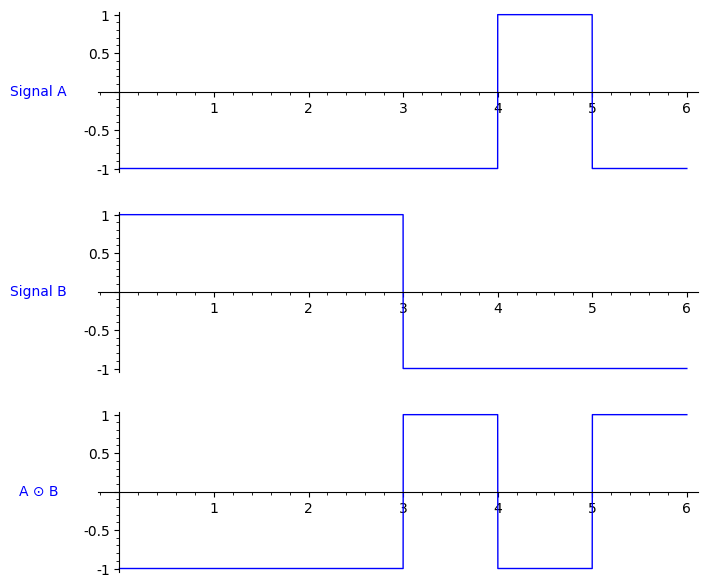
\includegraphics[width=0.7\linewidth]{Chapters/Introduction/signals_correlation}
\end{center}
\caption{\domingo{A graphical representation of two} vectors an their pointwise product with an unnormalized correlation between them of -2 (-1 -1 -1 +1 -1 +1)}
\label{introduction_signals_hadamard}
\end{figure}

\domingo{As represented in}Figure \ref{introduction_signals_hadamard}, \domingo{unnormalized correlation
can be performed using only integer arithmetics, multiplication and addition, thus becoming easier to implement using the resources  avaliable on a digital device.}










\subsection{Autocorrelation function}

Going on with the lecture of \citet{golomb_ref}, the autocorrelation function
is a measure of how the correlation behaves if, for a given sequence, a
circular shift is applied and \domingo{then }correlated with the original sequence for every
possible shift. It is defined for periodic sequences as follows:

\begin{definition}[Autocorrelation]\label{def:3}

Given the function C defined in Equation \eqref{eq:2} and n the length of the
sequence S

\begin{equation}\label{eq:3}
  shift(S, \tau)_i = S_{(i+\tau) \bmod n}
\end{equation}
\begin{equation}\label{eq:4}
  A(S)_{\tau} = C(S, shift(S, \tau)) = \sum_{i=1}^{n}S_{i}S_{(i+\tau) \bmod n}
\end{equation}

\end{definition}

\begin{figure}[ht!] % [h!] fuerza que el elemento se sitúe
                    % en la posición señalada, en vez de al
                    % comienzo de una página.
\begin{center}
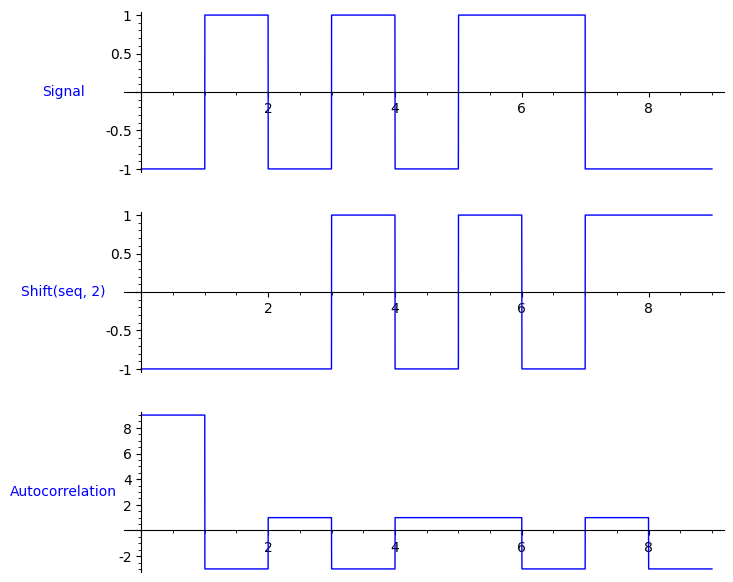
\includegraphics[width=0.7\linewidth]{Chapters/Introduction/signals_autocorrelation}
\end{center}
\caption{\domingo{A graphical representation of the autocorrelation of a sequence with  a shifted version of itself.}}
\label{introduction_signals_autocorrelation}
\end{figure}

\domingo{An example  is shown} in Figure
\ref{introduction_signals_autocorrelation} in which we can  \domingo{observe} 
some important properties of the autocorrelation \domingo{of sequences}:

\begin{theorem}\label{theorem:1.2.1}
  Given a sequence S, the autocorrelation value for \domingo{$\tau = 0$} is:
    \begin{equation}
      A(S)_{1}=C(S, S)=\sum_{i=1}^{n}S_{i}^2
    \end{equation}
\end{theorem}

\begin{corollary}
  Given the unnormalized autocorrelation of a sequence, we can
  normalize it by dividing it as follows:
  \begin{equation}
    A'(S)_{\tau} = \frac{A(S)_{\tau}}{A(S)_{\domingo{0}}}
  \end{equation}
\end{corollary}

\begin{proof}
  Using Equations \ref{eq:1} and \ref{eq:4}, we can normalize \ref{eq:4} as
  follows:

    $$A'(S)_{\tau} = C'(S, shift(S, \tau)) = \frac{C(S, shift(S, \tau))}{(\sum_{i=1}^{n} S_{i}^{2})^{\frac{1}{2}}(\sum_{i=1}^{n} S_{i+\tau}^{2})^\frac{1}{2}} = \frac{A(S)_{\tau}}{\sum_{i=1}^{n} S_{i}^{2}} = \frac{A(S)_{\tau}}{A(S)_{\domingo{0}}}$$

  Keep in mind that, even though $S_{i}^2$ and $S_{i+\tau}^2$ aren't the same element, the elements of the shifted version are the same as the original sequence so the total sum is the same.
\end{proof}

\begin{corollary}\label{autocorrelation:coro:1}
  Given the autocorrelation of a sequence, $A(S)_{\domingo{0}}$ will always be the maximum value of the autocorrelation.
\end{corollary}
\domingo{\textit{Esto no está claro, explicalo mejor}
\begin{property}
 Components of the autocorrelation vector belong to the same group as the
  original sequence.
\end{property}

Even though this seems a naive property, this will prove
useful when we introduce the algorithm based in the Fourier Transform to
compute the autocorrelation function.}









\subsection{Crosscorrelation function}

The crosscorrelation function measures how a sequence correlates with all
the posible shifts of another sequence. This function is useful to analyze if two signals can be mistaken one for another by a
receiver \domingo{when delays in time occur.}


\begin{definition}[Crosscorrelation]\label{def:4}
  Given C the correlation function defined in Equation \eqref{eq:2}, shift as the function defined in Equation \eqref{eq:3} and n the length of both sequences:
  \begin{equation}\label{eq:7}
    CC(S1, S2)_{\tau} = C(S1, shift(S2, \tau)) = \sum_{i=1}^{n}S1_{i}S2_{(i+\tau) \bmod n}
  \end{equation}
\end{definition}

\begin{figure}[ht!] % [h!] fuerza que el elemento se sitúe
                    % en la posición señalada, en vez de al
                    % comienzo de una página.
\begin{center}
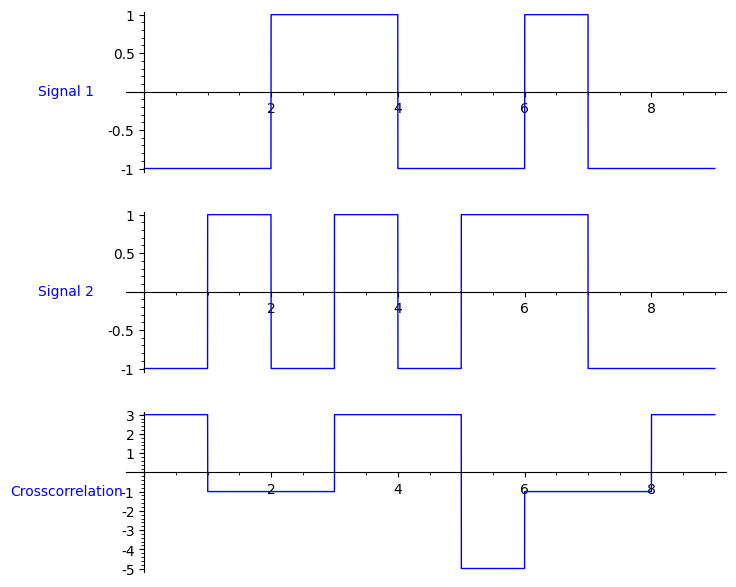
\includegraphics[width=0.7\linewidth]{Chapters/Introduction/signals_crosscorrelation}
\end{center}
\caption{\domingo{A graphical representation of the crosscorrelation between two sequences.}}
\label{introduction_signals_crosscorrelation}
\end{figure}

\begin{Definition}\label{lem:1}
  Given a sequence S, the crosscorrelation function  (CC) can bedefined in Equation
  \eqref{eq:7} with the autocorrelation function A defined in Equation \ref{eq:4}:
  \begin{equation}\label{eq:8}
    CC(S, S) = A(S)
  \end{equation}
\end{lemma}












\section{Pseudorandom noise \domingo{(PN)}}

Noise have a different meaning depending on the field of study in which is
used. In our case we are going to work with random vectors,
\domingo{which are defined as vectors whose components are realizations of independent and uniform distributed variables.
\cite{white_noise}}

Even though noise in general is usually seen as an unwanted \domingo{phenomena} that
limits the amount of information that can be transmitted through a
channel\cite{shannon_noise}, it is useful to study its properties, such as

%This practical applications exploit an important noise property:

\begin{property}
 \domingo{ The  expected value of the autocorrelation of a random vector  is zero}  for every component
  where $\tau \neq 0$ \cite{everett}
\end{property}

Taking a radar as an example, using \domingo{this property} can compute the distance
just by sending a \domingo{random sequence in the direction of }  a target and start correlating the
received signal with the original one. As the autocorrelation of
\domingo{random vector is different from zero} only  when the shift is \domingo{zero}, the \domingo{peak in the autocorrelation gives in } 
which time instant the signal has returned to the receiver. With that time instant, we can
get the round-trip time and then the actual distance \domingo{using} the
propagation speed of the wave.\\

In the case of GPS, the restrictions imposed to the \domingo{random} sequence are
stronger. First of all, as we will be \domingo{transmitting} several signals in the same
\domingo{frequency,} we need a set of \domingo{sequences} with good  \domingo{auto and} crosscorrelation properties
between them. In other words, the \domingo{maximum} crosscorrelation function between two given \domingo{sequences} must trend to \domingo{zero} in every component, except when \domingo{$\tau = 0$} and
both \domingo{sequences} are the same.\\

\domingo{Random sequences do not guarantee good properties of correlation, even} noise measured from natural phenomena
can generate sequences with poor correlation properties.\domingo{ As stated before, important}  technologies
depend on \domingo{sequences with these properties},  \domingo{Therefore it is necessary to develop methods that are efficient to create sequences} with properties similar to those of \domingo{random in} a deterministic and efficient
fashion.\\

This kind of sequences are called Pseudo Noise \domingo{(PN)}. \domingo{Although for most applications, the off peak autocorrelation and crosscorrelation should be equal to zero, it is conjetured that such sequence do not exist apart from length four. That is why pseudo noise are use in practical applications. Then a threshold is defined so that the system will not mistake intermediate values withe the peak in the autocorrelation. }


\begin{figure}[ht!] % [h!] fuerza que el elemento se sitúe
                    % en la posición señalada, en vez de al
                    % comienzo de una página.
\begin{center}
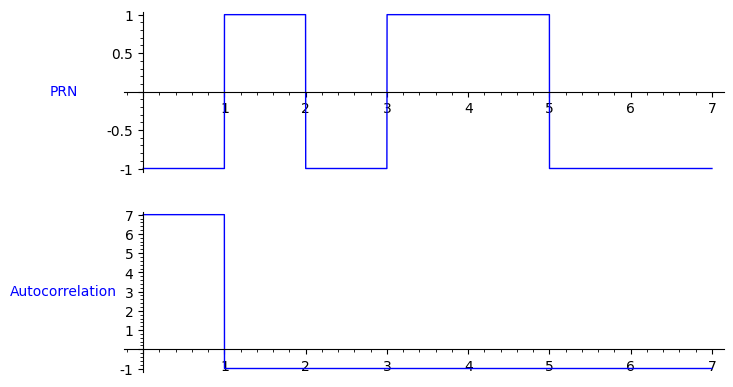
\includegraphics[width=0.7\linewidth]{Chapters/Introduction/signals_prn}
\end{center}
\caption{A pseudorandom noise sequence an it's autocorrelation function.
Notice that this PRN code isn't perfect noise.}
\label{introduction_signals_autocorrelation}
\end{figure}

% TODO Define family of sequences

% TODO Define flat autocorrelation
